% !TEX root = ../main.tex
\subsubsection{FMT Reconstruction}
\label{sssec::fmt_reconstruction}
    \begin{wrapfigure}{r}{0.50\textwidth}
        \centering\frame{
        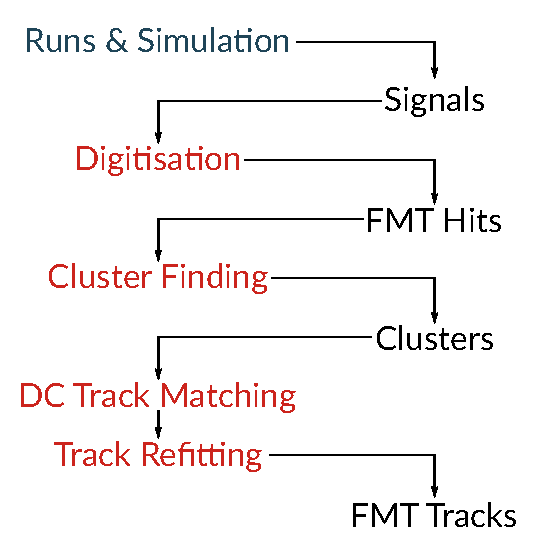
\includegraphics[width=\linewidth]{10fmt_recon.pdf}}
        \caption[FMT reconstruction summary]{FMT reconstruction summary.
        Data taking is coloured blue, data in black, and processes in red.
        Source: Own elaboration using \hyperlink{inkscape.org/}{Inkscape}.}
        \label{fig::fmt_recon}
    \end{wrapfigure}

    After a signal is detected on a readout strip and the data is stored, information is obtained from it from offline reconstruction.
    Being a tracker, FMT's reconstruction works in a fairly similar manner to DC's.

    First, after a signal is detected in a strip it is digitised, processed, and turned into an \textbf{FMT Hit}.
    A group of FMT hits is processed via a \textbf{Cluster Finding} algorithm, where a \textbf{Cluster} is defined as a group of hits that supposedly come from the same particle track.
    A group of clusters from different layers go through a \textbf{DC Track Matching} algorithm, where they are matched to DC tracks from DC Reconstruction.
    A \textbf{Track Refitting} algorithm is applied for each DC track using the clusters' data, updating them to re-fitted tracks, named \textbf{FMT tracks}.
    This whole process is summarised in figure \ref{fig::fmt_recon}.

\clearpage
